\documentclass[a4paper,11pt,twoside]{scrreprt}

\usepackage{txfonts}
\usepackage{graphicx}
\usepackage[utf8]{inputenc}
\usepackage[ngerman]{babel}
\usepackage[T1]{fontenc}

% Hilfsfunktion für Erkennenung der Erzeugung von PDF
\newif\ifpdf 
\ifx\pdfoutput\undefined
  \pdffalse
\else
  \ifx\pdfoutput\relax
    \pdffalse
  \else
    \ifnum\pdfoutput>0
      \pdftrue
    \else
      \pdffalse
    \fi
  \fi
\fi

\ifpdf
  \usepackage[ps2pdf]{thumbpdf}
  \usepackage[pdftex]{hyperref}
\else
  \usepackage[active]{srcltx}
\fi

\newcommand{\dctitle}{Literaturverwaltung}
\newcommand{\dcsubject}{Projektdokumentation}
\newcommand{\dcsubtitle}{Teilbeleg 1}
\newcommand{\dcauthor}{Simon Wunderlich}
\newcommand{\dcdate}{\today}

\ifpdf
\hypersetup{%
   pdfauthor={\dcsubject - \dcauthor}
   pdftitle={\dctitle}
   bookmarksnumbered=true,
   pdfstartview={FitH},
   colorlinks=true,
   linkcolor=black,
   plainpages = false
}
\fi
 % Metainformationen wie Titel, Autoren,...

\begin{document}
% Momentan (schlecht) handgestrickt - wenn jemand es mit \maketitle und den
% Autoren wie in Vorlage hinbekommt, bitte ändern

\begin{titlepage}
	\begin{center}\sffamily
		\vspace{15mm}
		
\includegraphics{tuclogo}
		\vfill
		{% Kopf des Titels
			\large Softwarepraktikum 2006\\[1.5ex]
		}
		\vfill \vfill

		%Titel
		\textbf{\Huge\dctitle}
		\vspace{1.5cm}
		
		% Subjekt
		\textbf{\Large\dcsubject}

		% Untertitel
		\textsc{\Large \dcsubtitle}
		\vfill \vfill
	\end{center}
	
	
	{%Autoren
		\begin{tabbing}
			\hspace{4.5cm}\=\textbf{Teamleiter:}\hspace{0.5cm}\=Simon~Wunderlich\\[2.0ex]
				\>\textbf{Mitglieder des Projektteams:}\\[1.5ex]
				\>            \>Andreas~Tröger \\[1.5ex]
				\>            \>Benedikt~Keil \\[1.5ex]
				\>            \>Frank~Wilhelm \\[1.5ex]
				\>            \>Florian~Scharl \\[1.5ex]
				\>            \>Sven~Eckelmann \\[4.0ex]
				\> \textbf{Praktikumsbetreuer:} Michael Rentzsch
		\end{tabbing}
	}
	\vfill
	
	{%Betreuer
		Chemnitz, den \dcdate
	}
\end{titlepage}
 % Titel des Dokuments mit Informationen aus meta

% nur zum arbeiten
\tableofcontents

%Kapitel
\chapter{Spezifikation der funktionellen Anforderungen}
\section{Produktbeschreibung}
Das Literaturverwaltungssystem LiMan unterst"utzt Autoren bei
ihrer Recherche durch ein intuitives Suchsystem. "Uber eine einfach
gehaltene Oberfl"ache werden alle Nutzungs- und Administrationsvorg"ange
abgewickelt. Durch das Websystem ist der Nutzer unabh"angig von Betriebssystem 
und Position.
\subsubsection*{Nutzungsumgebung}
Das System wird auf einem Webserver im Intranet oder 
Internet installiert, w"ahrend die Nutzer von ihren PCs mit
einem Webbrowser darauf zugreifen.
\subsubsection*{Nutzergruppe}
Es gibt 3 Nutzerebenen. Unregistrierte Nutzer k"onnen suchen und recherchieren,
Mitglieder d"urfen Literatur hinzuf"ugen und kommentieren, und Administratoren
d"urfen außerdem noch Mitglieder verwalten.


\section{Funktionelle Anforderungen}
\subsection{Umgebungsmodell}

\subsubsection{Ereignistabelle}
N = Nutzer, M = registriertes Mitglied, A = Administrator \\
M kann zusätzlich zu seinen, alle Ereignisse von N auslösen. A kann ebenso alle Ereignisse von M und N auslösen.

\begin{longtable}{|c|p{9.0em}|p{10.5em}|l|}
\hline
Nr & Ereignis & Datenfluß im System & Antwort des Systems \\
\hline\hline
\endhead

1. & N ruft neu hinzugefügte Literatur ab & - & Letzte\_Literatur \\\hline
2. & N sucht Literatur & Suchbegriff & Suchtreffer \\\hline
3. & N wählt Literatur & Literatur\_Nr & Literatur\_Info \\\hline
4. & N exportiert Literatur & Exportanfrage &  BibTeX-Datei \\\hline
5. & M legt Literatur an & Literaturdaten & Bestätigung\_Literaturanlegen \\\hline
6. & M ändert Literatur & Literatur & Bestätigung\_Literaturändern\\\hline
7. & M löscht Literatur & Literatur\_Nr & Bestätigung\_Literaturlöschen \\\hline
8. & M ändert Mitglied & Mitglied & Bestätigung\_Mitgliedändern \\\hline
9. & M legt Kommentar an & Kommentardaten & Bestätigung\_Kommentaranlegen \\\hline
10. & M ändert Kommentar & Kommentar & Bestätigung\_Kommentarändern \\\hline
11. & M löscht Kommentar & Kommentar\_Nr & Bestätigung\_Kommentarlöschen \\\hline
12.& M importiert BibTeX & BibTeX-Datei & Bestätigung\_BibTeXImport \\\hline
13.& A legt Mitglied an & Mitgliedsdaten & Bestätigung\_Mitgliedanlegen \\\hline
14.& A löscht Mitglied & Mitglieds\_Nr & Bestätigung\_Mitgliedlöschen \\\hline
15.& A ruft Mitglieder ab & - & Mitgliederliste \\\hline
\end{longtable}

\newpage % Viele Bilder so skaliert, dass sie ordentlich auf A4-Seiten passen
\subsubsection{Kontextdiagramm}

%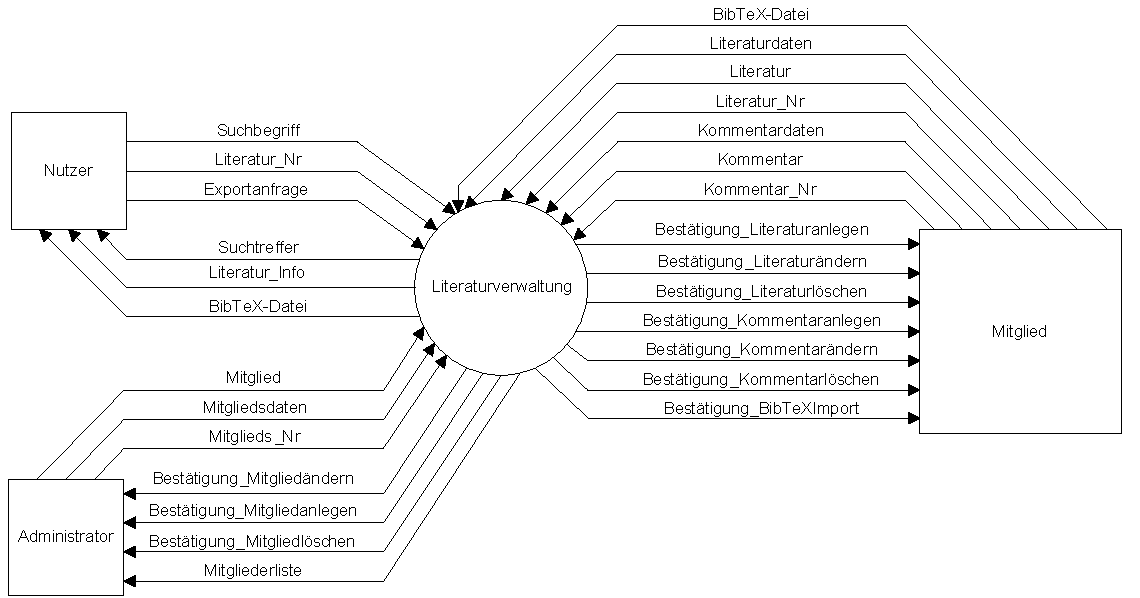
\includegraphics[scale=0.5]{kontextdiagramm}
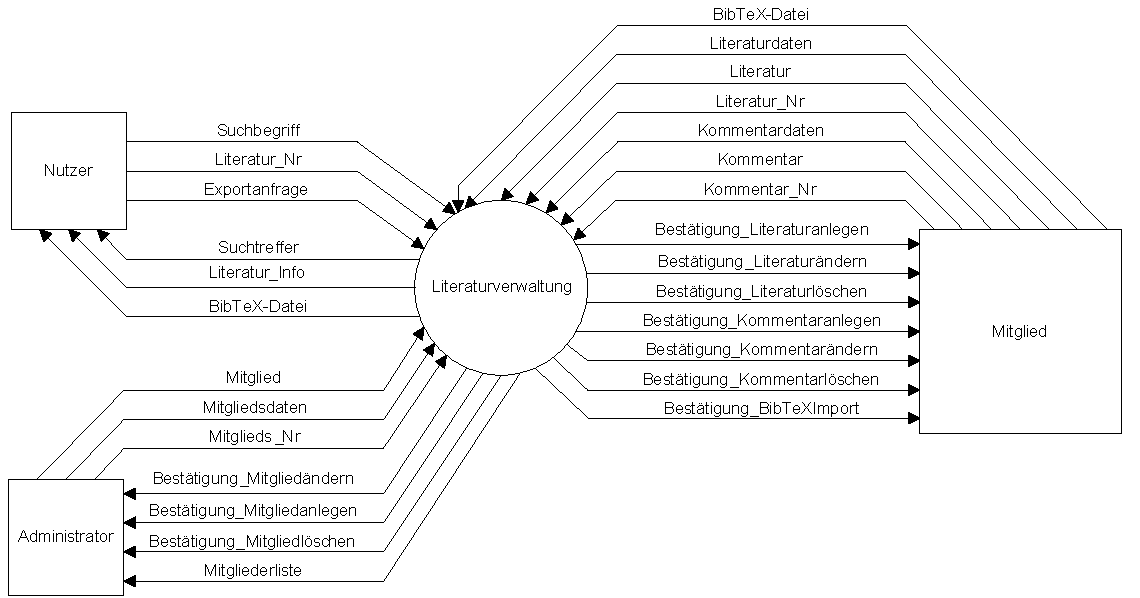
\includegraphics[scale=0.75]{kontextdiagramm}

\subsection{Verhaltensmodell}
\subsubsection{Grobes Verhaltensmodell (vergröbertes primäres Verhaltensmodell)}
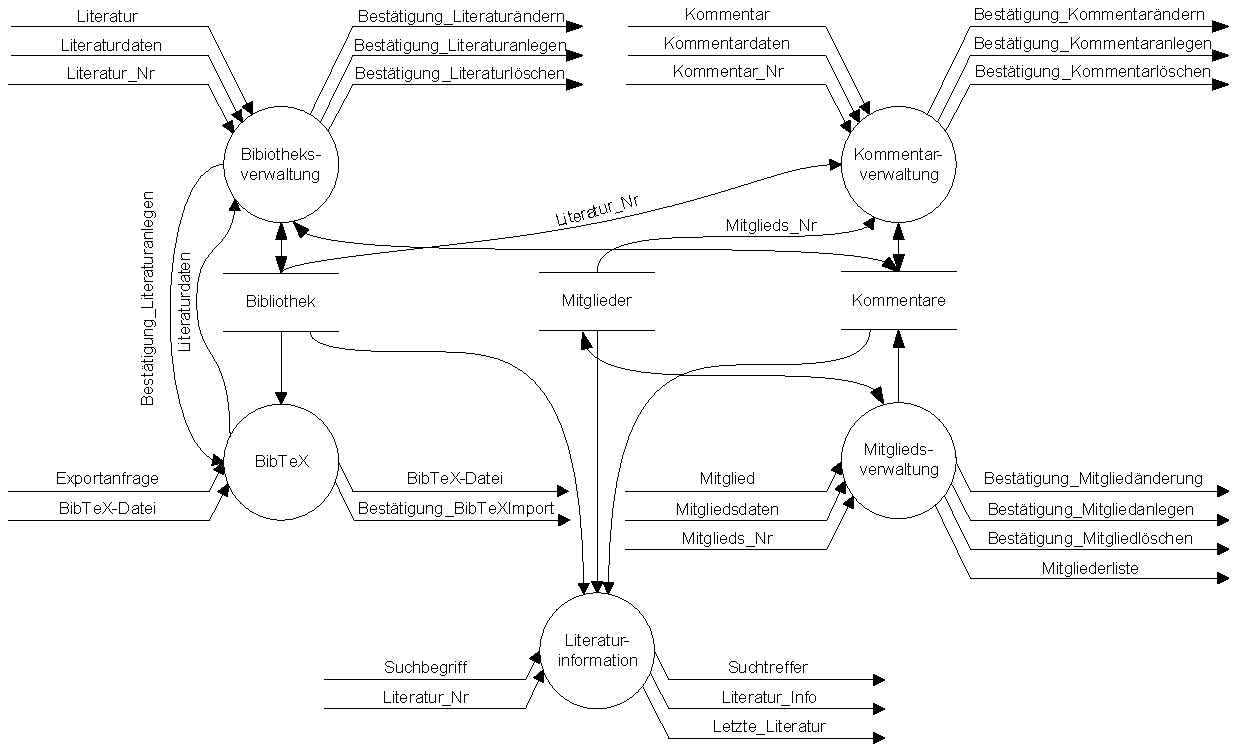
\includegraphics[scale=0.70]{grobes_verhaltensmodell}

\subsubsection{Primäres Verhaltensmodell}
\paragraph{Teilmodell BibTeX}
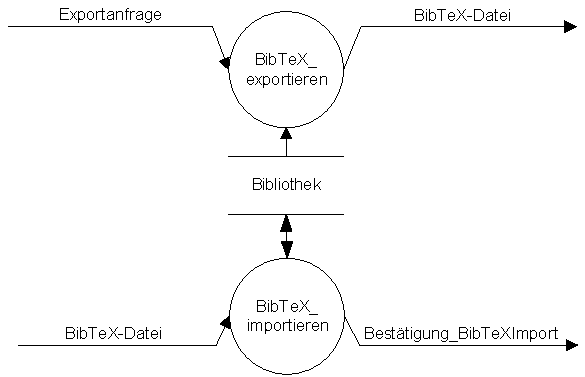
\includegraphics[scale=1.0]{teilmodell_bibtex}

\paragraph{Teilmodell Literaturinformation}
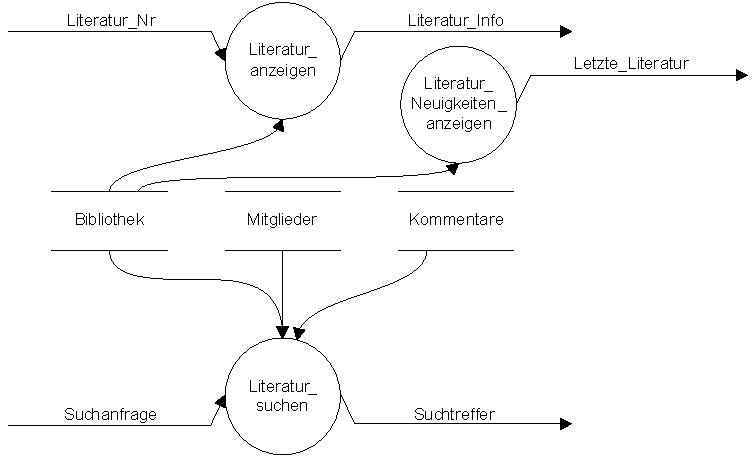
\includegraphics[scale=1.0]{teilmodell_literaturinformation}

\paragraph{Teilmodell Literaturverwaltung}
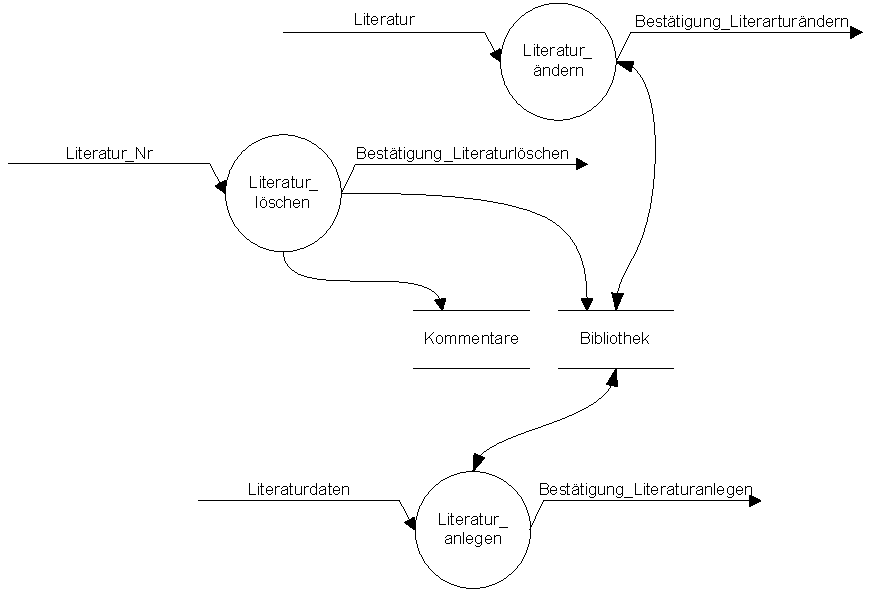
\includegraphics[scale=0.93]{teilmodell_bibliotheksverwaltung}

\paragraph{Teilmodell Kommentarverwaltung}
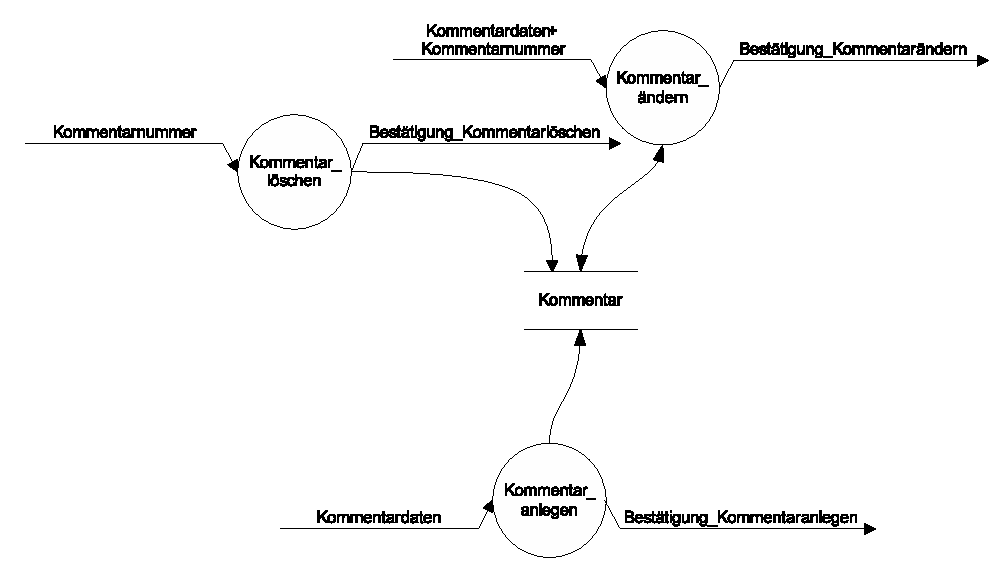
\includegraphics[scale=0.88]{teilmodell_kommentarverwaltung}

\paragraph{Teilmodell Mitgliederverwaltung}
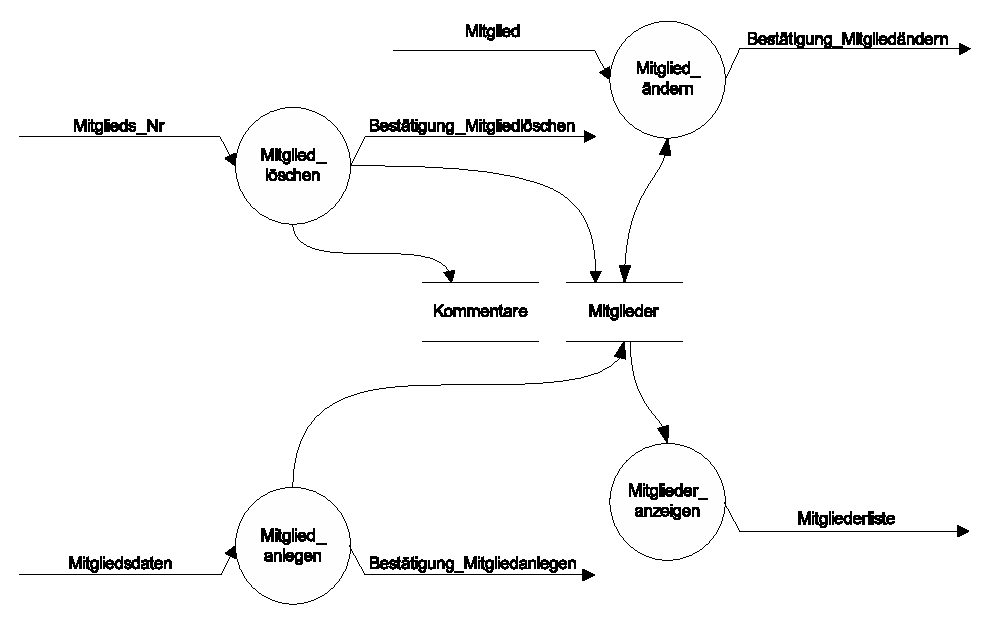
\includegraphics[scale=0.85]{teilmodell_mitgliederverwaltung}
\newpage

\subsubsection{Datenkatalog}
\begin{longtable}{|l|p{8.5cm}|}
\hline
Element & Strukturbeschreibung \\
\hline\hline
\endhead

\emph{Bibliothek} & \{Literatur\} \\
\hline
Literatur & @Literatur\_Nr + Art + Titel + (Jahr) + (Verlag) + (ISBN) + (Beschreibung) + (Ort) + (Stichworte) \\
\hline
Literatur\_Nr & gZahl *6stellig, 000001 $\leq$ Literatur\_Nr $\leq$ 999999* \\
\hline
Art & ['' Buch'' | '' Artikel '' | '' Broschüre '' | '' Protokoll '' | '' Anleitung '' | '' Diplomarbeit '' | '' Dissertation '' | '' Techn. Bericht '' | '' Unveröffentlicht '' | '' Sonstiges ''] \\
\hline
Titel & Zeichenkette40 \\
\hline
Jahr & gZahl \\
\hline
Verlag & Zeichenkette40 \\
\hline
ISBN & Zeichenkette20 \\
\hline
Beschreibung & Zeichenkette250 \\
\hline
Ort & Zeichenkette40 \\
\hline
Stichworte & Zeichenkette100 \\
\hline\hline

\emph{Autoren} & \{Autor\} \\
\hline
Autor & @Autor\_Nr + \{Autorname\} \\
\hline
Autor\_Nr & gZahl *6stellig, 000001 $\leq$ Autor\_Nr $\leq$ 999999* \\
\hline
Autorname & Zeichenkette40 \\
\hline\hline

\emph{Kommentare} & \{Kommentar\} \\
\hline
Kommentar & @Kommentar\_Nr + Kommentartext + Literatur\_Nr + Mitglieds\_Nr\\
\hline
Kommentar\_Nr & gZahl *6stellig, 000001 $\leq$ Kommentar\_Nr $\leq$ 999999* \\
\hline
Kommentartext & Zeichenkette400 \\
\hline\hline

\emph{Mitglieder} & \{Mitglied\} \\
\hline
Mitglied  & @Mitglieds\_Nr  + Name + Vorname + Login + Passwort + Rechte + E-Mail\\
\hline
Mitglieds\_Nr & gZahl *6stellig, 000001 $\leq$ Mitglieds\_Nr $\leq$ 999999* \\ 
\hline
Name & Zeichenkette20 \\
\hline
Vorname & Zeichenkette20 \\
\hline
E-Mail & Zeichenkette350 \\
\hline
Login & Zeichenkette12 \\
\hline
Passwort & Zeichenkette12 \\
\hline
Rechte & [``Benutzer'' $\mid $``Administrator``] \\
\hline\hline

Mitgliedsdaten & Name + Vorname + Login + Passwort + Rechte + E-Mail\\
\hline
Literaturdaten & Art + Titel + Autorname + (Jahr) + (Verlag) + (ISBN) + (Beschreibung) + (Ort) + (Stichworte) \\
\hline
Kommentardaten & Literatur\_Nr + Mitglieds\_Nr + Kommentartext \\
\hline
BibTeX-Datei & *Datei im Bibtexformat* \\
\hline
Suchbegriff & Zeichenkette100 \\
\hline
Exportanfrage & Literatur\_Nr \\
\hline\hline

Bestätigung\_BibTeXImport & Literatur\_Nr + Zeichenkette ''Importieren vorgenommen`` \\
\hline
Bestätigung\_Literaturanlegen & Literatur\_Nr + Zeichenkette ''Anlegen vorgenommen`` \\
\hline
Bestätigung\_Literaturändern & Literatur\_Nr + Zeichenkette ''Änderung vorgenommen`` \\
\hline
Bestätigung\_Literaturlöschen & Literatur\_Nr + Zeichenkette ''Löschen vorgenommen`` \\
\hline
Bestätigung\_Kommentaranlegen & Kommentar\_Nr + Zeichenkette ''Anlegen vorgenommen`` \\
\hline
Bestätigung\_Kommentarändern & Kommentar\_Nr + Zeichenkette ''Änderung vorgenommen`` \\
\hline
Bestätigung\_Kommentarlöschen & Kommentar\_Nr + Zeichenkette ''Löschen vorgenommen`` \\
\hline
Bestätigung\_Mitgliedanlegen & Mitglieds\_Nr + Zeichenkette ''Anlegen vorgenommen`` \\
\hline
Bestätigung\_Mitgliedändern & Mitglieds\_Nr + Zeichenkette ''Änderung vorgenommen`` \\
\hline
Bestätigung\_Mitgliedlöschen & Mitglieds\_Nr + Zeichenkette ''Löschen vorgenommen`` \\
\hline
Suchtreffer & \{Literatur\_Nr + Titel + Autorname + Verlag + ISBN\}\\
\hline
Letzte\_Literatur & \{Literatur\_Nr + Titel + Autorname + Verlag + ISBN\}\\
\hline
Mitgliederliste & \{Mitglieds\_Nr + Name + Vorname\}\\
\hline
\end{longtable}

\subsubsection{Beziehungen zwischen Speichern (ERD)}
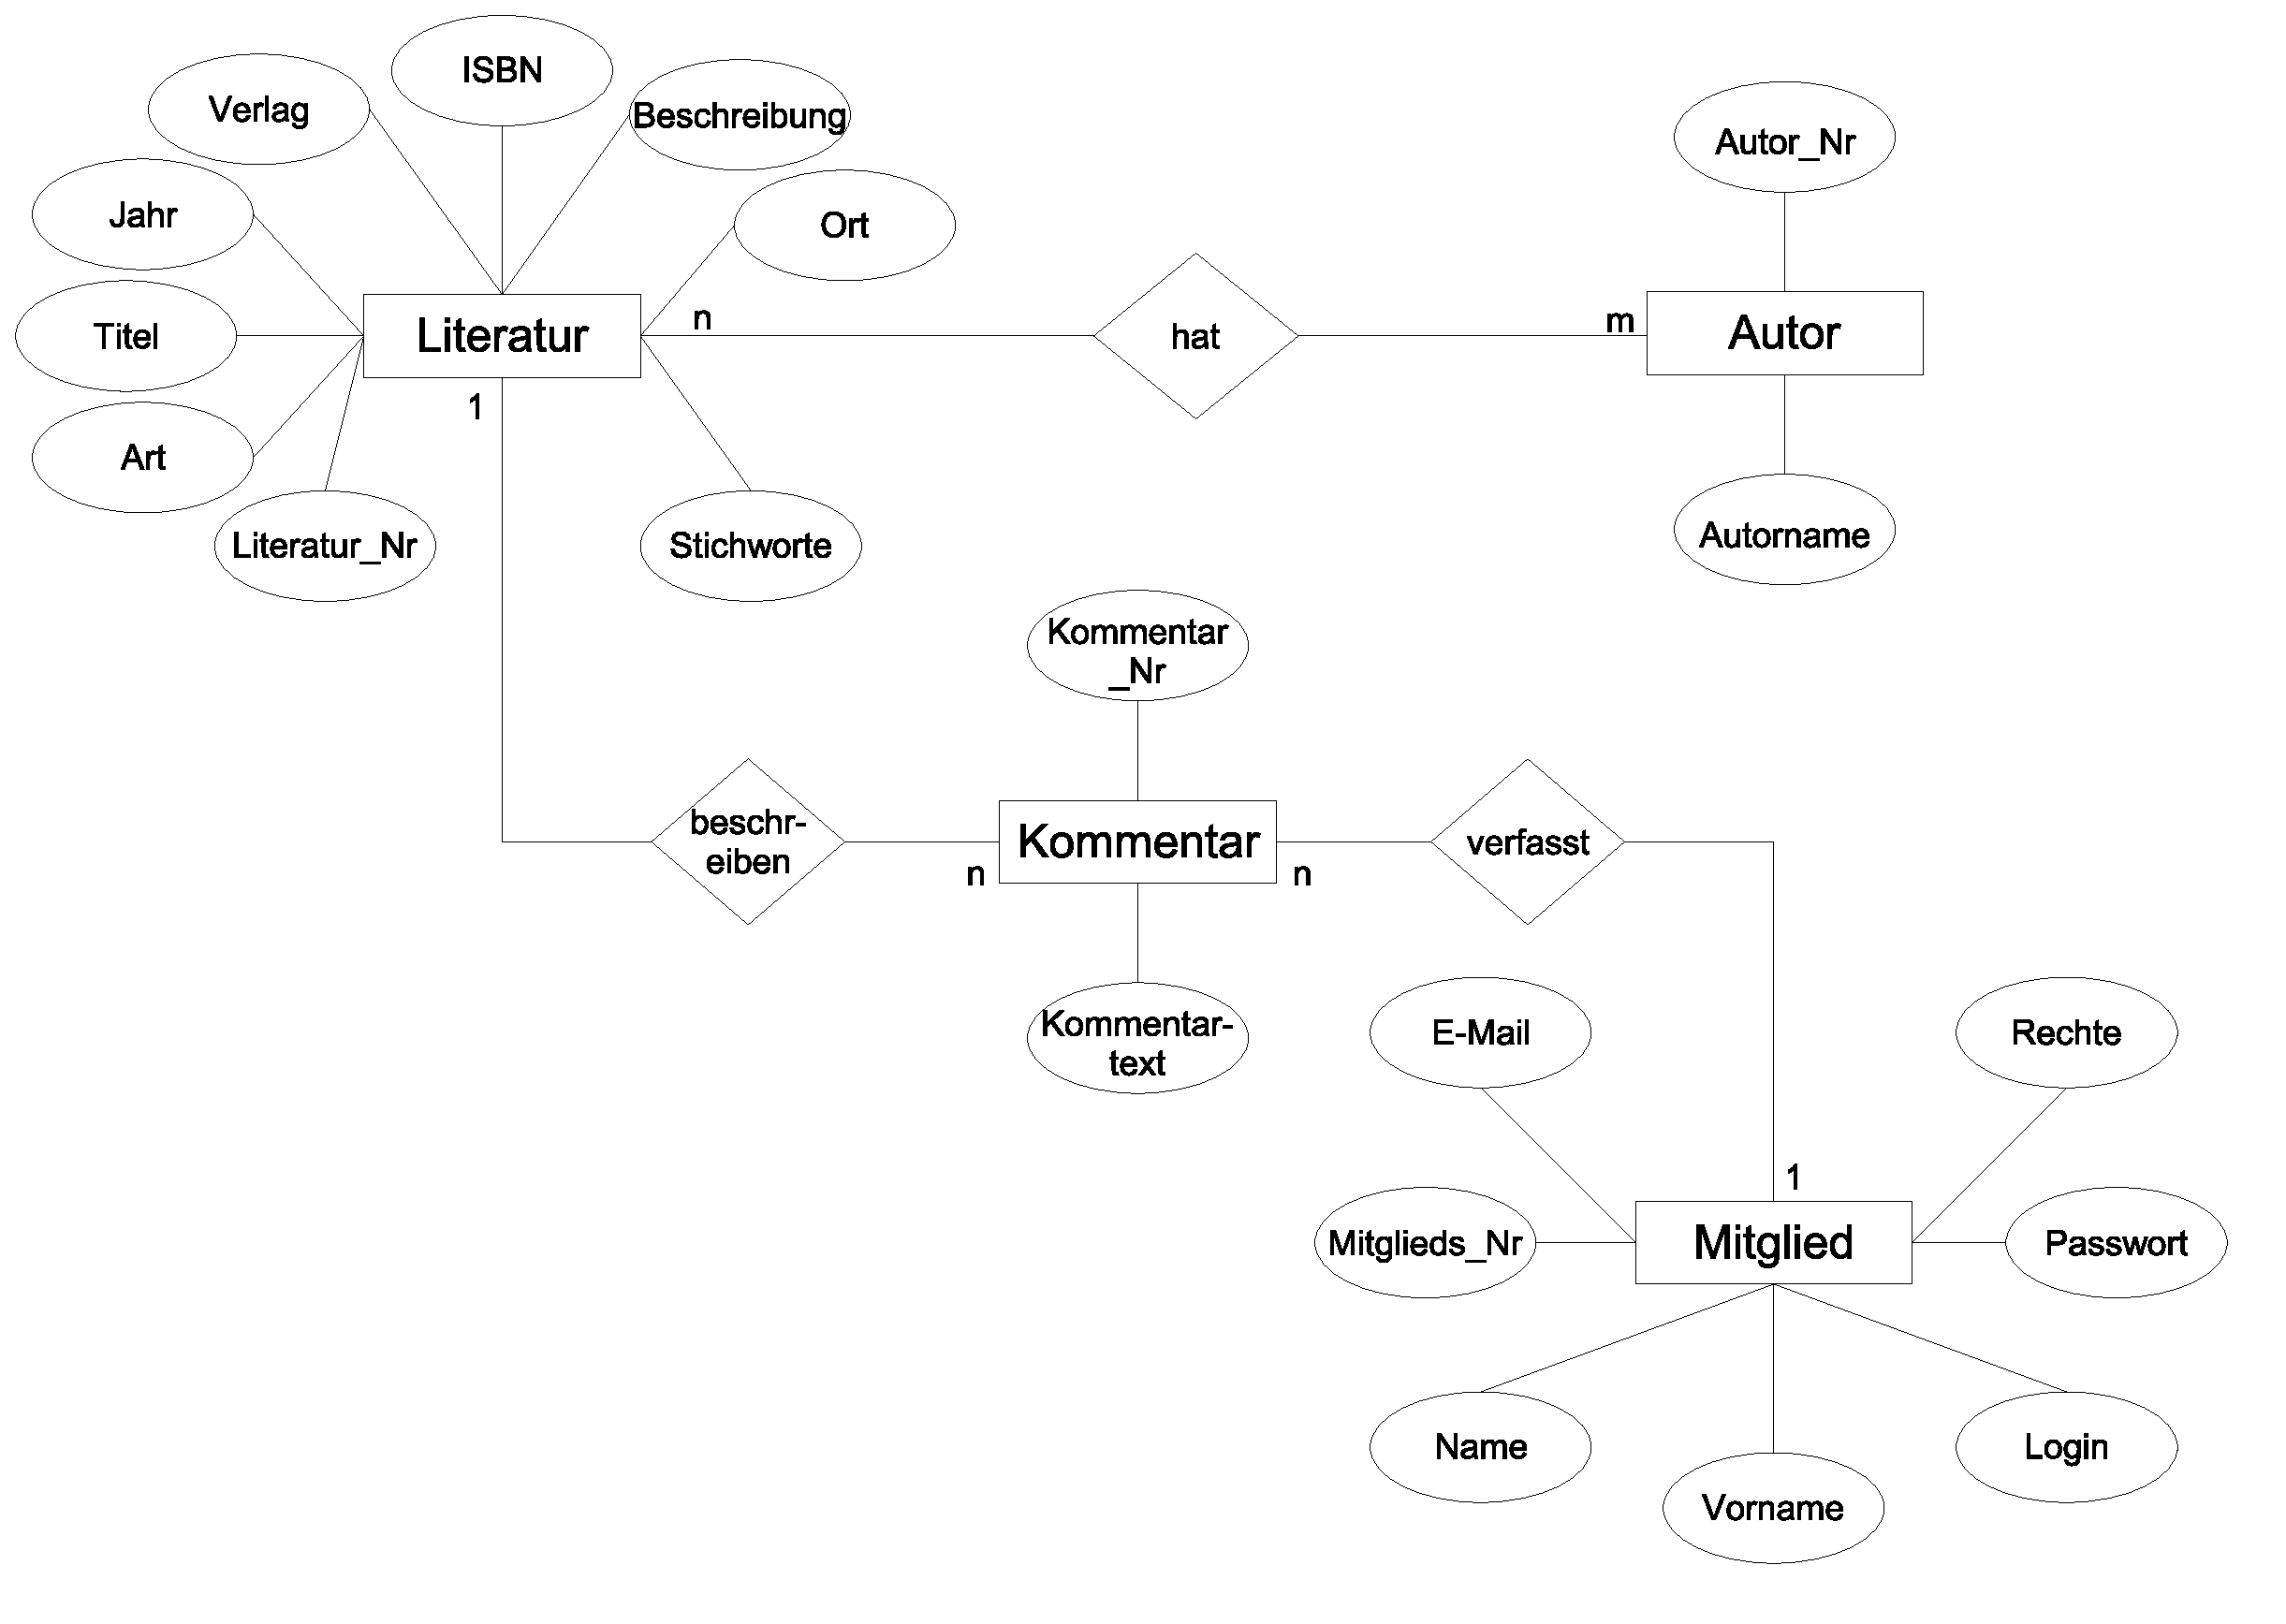
\includegraphics[scale=0.36]{erd1}

\subsubsection{Prozessspezifikation}
% Literatur_anlegen
\paragraph{Literatur\_anlegen}
\begin{tabular}[t]{p{9.5cm}ll}
\textbf{Prozess}: Literatur\_anlegen  	&\textbf{Datum}:      &21.04.2006\\
					&\textbf{Bearbeiter}: &Frank Wilhelm\\
\end{tabular}

\hrulefill\\
\textbf{Voraussetzung}: Benutzer ist angemeldet. Bibliothek ist nicht voll.
\begin{verbatim}
 BEGIN
   Finde in Bibliothek Literatur
         mit Literatur.Titel = Literaturdaten.Titel
         und Literatur.Autor = Literaturdaten.Autor;
 
   IF gefunden THEN
   BEGIN
     Zeige Warnung 101
     IF not bestätigt THEN
       Abbrechen
   END
   
   Finde in Autoren Autor
         mit Autor.Name = Literaturdaten.Autor.Name;
         
   IF gefunden THEN
     Literaturdaten.Autor := Autor
   ELSE
   BEGIN
     Lege in Autoren Autor mit Literaturdaten.Autor.Name an
     Literaturdaten.Autor := Autor
   END
   
   Lege in Bibliothek Literatur mit Literaturdaten an
   Setze Bestätigung_Literaturanlegen
 END
\end{verbatim}
\hrulefill



% Literatur_ändern
\paragraph{Literatur\_ändern}
\begin{tabular}[t]{p{9.5cm}ll}
\textbf{Prozess}: Literatur\_ändern  	&\textbf{Datum}:      &21.04.2006\\
					&\textbf{Bearbeiter}: &Frank Wilhelm\\
\end{tabular}

\hrulefill\\
\textbf{Voraussetzung}: Benutzer ist angemeldet.
\begin{verbatim}
 BEGIN
   Finde in Autoren Autor
         mit Autor.Name =  Literatur.Autor.Name;
         
   IF gefunden THEN
      Literatur.Autor := Autor
   ELSE
   BEGIN
     Lege in Autoren Autor mit Literaturdaten.Autor.Name an
     Literatur.Autor := Autor
   END
   
   Setze in Bibliothek Literatur_Eintrag
         mit Literatur_Eintrag.Literatur_Nr = Literatur.Literatur_Nr
         auf Literatur;
  
   IF erfolgreich THEN
     Setze Bestätigung_Literaturändern
   ELSE
     Setze Fehler 102
 END
\end{verbatim}
\hrulefill



% Literatur_löschen
\paragraph{Literatur\_löschen}
\begin{tabular}[t]{p{9.5cm}ll}
\textbf{Prozess}: Literatur\_löschen  	&\textbf{Datum}:      &21.04.2006\\
					&\textbf{Bearbeiter}: &F. Wilhelm\\
\end{tabular}

\hrulefill\\
\textbf{Voraussetzung}: Benutzer ist angemeldet.
\begin{verbatim}
 BEGIN
   Lösche in Bibliothek Literatur mit Literatur.Literatur_Nr = 
                                      Literatur_Nr;

   IF erfolgreich THEN
     Lösche in Kommentare Kommentar mit Kommentar.Literatur_Nr = 
                                        Literatur_Nr

     Lösche in Autoren Autor mit Autor ohne Literatur

     Setze Bestätigung_Literaturlöschen
   ELSE
     Setze Fehler 103
 END
\end{verbatim}
\hrulefill
% BibTeX_importieren
\paragraph{BibTeX\_importieren}
\begin{tabular}[t]{p{9.5cm}ll}
\textbf{Prozess}: BibTeX\_importieren  	&\textbf{Datum}:      &21.04.2006\\
					&\textbf{Bearbeiter}: &Frank Wilhelm\\
\end{tabular}

\hrulefill\\
\textbf{Voraussetzung}:
\begin{verbatim}
 BEGIN
   Daten := deserialisiere BibTeX_Datei;
   
   IF lesen_erfolgreich THEN
   BEGIN
     Buch_anlegen( Daten )
     
     IF anlegen_erfolgreich THEN
       Setze Bestätigung_BibTeXImport
   END
   ELSE
     Setze Fehler 101
 END
\end{verbatim}
\hrulefill


% BibTeX_exportieren
\paragraph{BibTeX\_exportieren}
\begin{tabular}[t]{p{9.5cm}ll}
\textbf{Prozess}: BibTeX\_exportieren  	&\textbf{Datum}:      &21.04.2006\\
					&\textbf{Bearbeiter}: &Frank Wilhelm\\\\
\end{tabular}

\hrulefill\\
\textbf{Voraussetzung}:
\begin{verbatim}
 BEGIN
   Daten := Finde in Buecher Literatur mit Literatur.Buch_Nr = \
              Exportanfrage.Buch_Nr;
  
   IF gefunden THEN
     BibTeX_Datei := Serialisiere Daten
   ELSE
     Setze Fehler 102
 END
\end{verbatim}

\hrulefill


% Kommentar_anlegen
\paragraph{Kommentar\_anlegen}
\begin{tabular}[t]{p{9.5cm}ll}
\textbf{Prozess}: Kommentar\_anlegen  	&\textbf{Datum}:      &21.04.2006\\
					&\textbf{Bearbeiter}: &S. Eckelmann\\
\end{tabular}

\hrulefill\\
\textbf{Voraussetzung}: Benutzer ist angemeldet. Kommentardaten.Mitglieds\_Nr ist die Nummer des aktuell angemeldeten Nutzers. Kommentare ist nicht voll.
\begin{verbatim}
  BEGIN
   Finde in Bibliothek Literatur
         mit Literatur.Titel = Kommentardaten.Buch_Nr
   und Finde in Literatur.Autor = Literaturdaten.Autor;
 
   IF gefunden THEN
   BEGIN
     Finde in Kommentare Kommentar
           mit Kommentar.Mitglieds_Nr = Kommentardaten.Mitglieds_Nr
           und Kommentar.Literatur_Nr = Kommentardaten.Literatur_Nr

     IF gefunden THEN
       Setze Fehler 301
     ELSE
     BEGIN
       Lege in Kommentare Kommentar mit Kommentardaten an
       Setze Bestätigung_Kommentaranlegen
     END

   END
 END
\end{verbatim}
\hrulefill



% Kommentar_ändern
\paragraph{Kommentar\_ändern}
\begin{tabular}[t]{p{9.5cm}ll}
\textbf{Prozess}: Kommentar\_ändern  	&\textbf{Datum}:      &21.04.2006\\
					&\textbf{Bearbeiter}: &S. Eckelmann\\
\end{tabular}

\hrulefill\\
\textbf{Voraussetzung}: Benutzer ist angemeldet. Kommentardaten.Mitglieds\_Nr ist die Nummer des aktuell angemeldeten Nutzers (außer er ist Administrator)
\begin{verbatim}
 BEGIN
   Setze in Kommentare Kommentar_Eintrag
         mit Kommentar_Eintrag.Kommentar_Nr = Kommentar.Kommentar_Nr
         auf Kommentar;
  
   IF erfolgreich THEN
     Setze Bestätigung_Kommentarändern
   ELSE
     Setze Fehler 302
 END
\end{verbatim}
\hrulefill



% Kommentar_löschen
\paragraph{Kommentar\_löschen}
\begin{tabular}[t]{p{9.5cm}ll}
\textbf{Prozess}: Kommentar\_löschen  	&\textbf{Datum}:      &21.04.2006\\
					&\textbf{Bearbeiter}: &S. Eckelmann\\
\end{tabular}

\hrulefill\\
\textbf{Voraussetzung}: Benutzer ist angemeldet. Kommentardaten.Mitglieds\_Nr ist die Nummer des aktuell angemeldeten Nutzers (außer er ist Administrator)
\begin{verbatim}
 BEGIN
   Lösche in Kommentare Kommentar mit Kommenar.Kommentar_Nr = 
                                      Kommentar_Nr;
   
   IF erfolgreich THEN
     Setze Bestätigung_Kommentarlöschen
   ELSE
     Setze Fehler 303
 END
\end{verbatim}
\hrulefill
% Literatur_anzeigen
\paragraph{Literatur\_anzeigen}
\begin{tabular}[t]{p{9.5cm}ll}
\textbf{Prozess}: Literatur\_anzeigen  	&\textbf{Datum}:      &21.04.2006\\
					&\textbf{Bearbeiter}: &S. Eckelmann\\
\end{tabular}

\hrulefill\\
\textbf{Voraussetzung}: -
\begin{verbatim}
 BEGIN
   Finde in Bibliothek Literatur
         mit Literatur.Literatur_Nr = Literatur_Nr

   IF gefunden THEN
   BEGIN
     Finde in Kommentare Kommentar
           mit Kommentar.Literatur_Nr =  Literatur_Nr

     IF gefunden THEN
       Setze Literatur_Info := gefundene_Literatur
                             + gefundene_Kommentare
     ELSE
       Setze Literatur_Info := gefundene_Literatur
   END
   ELSE
     Setze Fehler 401
 END
\end{verbatim}
\hrulefill

% Literatur_Neuigkeiten_anzeigen
\paragraph{Literatur\_Neuigkeiten\_anzeigen}
\begin{tabular}[t]{p{9.5cm}ll}
\textbf{Prozess}: Literatur\_Neuigkeiten\_anzeigen  	&\textbf{Datum}:      &21.04.2006\\
					&\textbf{Bearbeiter}: &S. Eckelmann\\
\end{tabular}

\hrulefill\\
\textbf{Voraussetzung}: -
\begin{verbatim}
 BEGIN
   Finde 10 Einträge mit den höchsten Literatur_Nr in Bibliothek

   IF erfolgreich THEN
      Setze Letzte_Literatur := gefundene_Literatur
   ELSE
      Setze Fehler 402
 END
\end{verbatim}
\hrulefill


% Literatur_suchen
\paragraph{Literatur\_suchen}
\begin{tabular}[t]{p{9.5cm}ll}
\textbf{Prozess}: Literatur\_suchen  	&\textbf{Datum}:      &21.04.2006\\
					&\textbf{Bearbeiter}: &S. Eckelmann\\
\end{tabular}

\hrulefill\\
\textbf{Voraussetzung}: -
\begin{verbatim}
 BEGIN
   Finde in Bibliothek Literatur
         die Suchanfrage erfüllt
   
   IF gefunden THEN
     Setz Suchtreffer := gefundene_Literatur
   ELSE
     Setze Fehler 403
 END
\end{verbatim}
\hrulefill
% Mitglieder_anzeigen
\paragraph{Mitglieder\_anzeigen}
\begin{tabular}[t]{p{9.5cm}ll}
\textbf{Prozess}: Mitglieder\_anzeigen 	&\textbf{Datum}:      &21.04.2006\\
					&\textbf{Bearbeiter}: &S. Eckelmann\\
\end{tabular}

\hrulefill\\
\textbf{Voraussetzung}: Benutzer muss als Administrator angemeldet sein.
\begin{verbatim}
 BEGIN
   Finde alle in Mitglieder

   IF erfolgreich THEN
      Setze Mitgliederliste := gefundene_Mitglieder
   ELSE
      Setze Fehler 501
 END
\end{verbatim}
\hrulefill

% Mitglied_anlegen
\paragraph{Mitglied\_anlegen}
\begin{tabular}[t]{p{9.5cm}ll}
\textbf{Prozess}: Mitglied\_anlegen  	&\textbf{Datum}:      &21.04.2006\\
					&\textbf{Bearbeiter}: &S. Eckelmann\\
\end{tabular}

\hrulefill\\
\textbf{Voraussetzung}: Benutzer muss als Administrator angemeldet sein. Es darf keinen anderes Mitglied mit gleichen Login geben (von Datenbank abgefangen).
\begin{verbatim}
 BEGIN
   Bestimme Hash des Passworts
   Lege in Mitglieder Mitglied mit Mitgliedsdaten an

   IF gefunden THEN
     Setze Fehler 502
   ELSE
     Setze Bestätigung_Mitgliedanlegen
 END
\end{verbatim}
\hrulefill



% Mitglied_ändern
\paragraph{Mitglied\_ändern}
\begin{tabular}[t]{p{9.5cm}ll}
\textbf{Prozess}: Mitglied\_ändern  	&\textbf{Datum}:      &21.04.2006\\
					&\textbf{Bearbeiter}: &S. Eckelmann\\
\end{tabular}

\hrulefill\\
\textbf{Voraussetzung}: Benutzer ist angemeldet. Mitglied.Mitglieds\_Nr ist die Nummer des aktuell angemeldeten Nutzers (außer er ist Administrator)
\begin{verbatim}
  BEGIN
   Bestimme Hash des Passworts, wenn geändert
   Setze in Mitglieder Mitglied_Eintrag
         mit Mitglied_Eintrag.Mitglieds_Nr = Mitglied.Mitglieds_Nr
         auf Mitglied;
  
   IF erfolgreich THEN
     Setze Bestätigung_Mitgliedändern
   ELSE
     Setze Fehler 503
 END
\end{verbatim}
\hrulefill



% Mitglied_löschen
\paragraph{Mitglied\_löschen}
\begin{tabular}[t]{p{9.5cm}ll}
\textbf{Prozess}: Mitglied\_löschen  	&\textbf{Datum}:      &21.04.2006\\
					&\textbf{Bearbeiter}: &S. Eckelmann\\
\end{tabular}

\hrulefill\\
\textbf{Voraussetzung}: Benutzer muss als Administrator angemeldet sein.
\begin{verbatim}
 BEGIN
   Lösche in Mitglieder Mitglied mit Mitglied.Mitglieds_Nr = 
                                     Mitglieds_Nr;

   IF erfolgreich THEN
     Lösche in Kommentare Kommentar mit Kommentar.Mitglieds_Nr = 
                                        Mitglieds_Nr

     Setze Bestätigung_Mitgliedlöschen
   ELSE
     Setze Fehler 504
 END
\end{verbatim}
\hrulefill

\subsection{Definition der Nutzerschnittstelle}

Durch das Websystem ist die Nutzerschnittstelle beschr"ankt auf die Darstellung im Browser. Dadurch kann die Darstellung
leicht bei verschiedenen Browser und Betriebssystemen variieren. Die Eingabefelder und Kn"opfe werden im Stil des 
Betriebssystems dargestellt, sodass der Benutzer stets seine gewohnte Umgebung vorfinden kann. Ebenso kann man mittels der Optionen
des Browser Schriftgr"o"se und andere visuelle Einstellungen ver"andern. Das Grundlayout bleibt jedoch immer erhalten
und richtet sich unter anderem auch nach der Gr"o"se des ge"offneten Browserfensters.\\
\\
Das Layout teilt sich in einen Navigations-/"Ubersichtsteil auf der linken Seite der unabh"angig von der Auswahl immer
zu sehen ist. Hier findet sich die Navigation, die Suchmaske f"ur die Suchfunktion sowie Authentifikationsmaske zum Login.
Auf der rechten, gr"o"seren Seite befindet sich der Inhalt der aktuell aufgerufenen Funktion.\\
\\
Die Benutzung beginnt gew"ohnlich auf der Literaturliste (Startseite), jede Seite kann aber "uber direkte
Ansteuerung mittels der Adresszeile des Browser oder auch Bookmarks abgerufen werden.\\

\subsubsection{Ein- und Ausgabegeräte}
F"ur die Eingabe wird ein vernetzter PC mit Tastatur und Maus vorrausgesetzt.\\
Die Ausgabe erfolgt stets "uber einen Farbmonitor.
\newpage
\subsubsection{Navigationsleiste}
\begin{floatingfigure}[r]{0.4\textwidth}
\centering
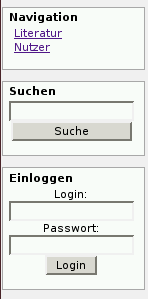
\includegraphics[scale=0.6]{navigation.png} 
\end{floatingfigure}

Diese Leiste findet man unabh"angig vom Inhalt immer auf der linken Seite.
Unter {\bf Navigation} findet man die Unterpunkte ``Literatur'' und ``Nutzer'', die zu den entsprechenden Listen f"uhren.\\
\\
{\bf Suchen} erlaubt die Eingabe eines Suchbegriffes, mit dem Knopf ``Suche'' wird der Vorgang gestartet. 
Das Ergebnis findet sich dann im Inhaltsbereich auf der rechten Seite.\\
\\
Zum {\bf Einloggen} gibt man seinen Nutzerkennzeichen und Passwort ein. Ist man bereits eingeloggt, ist hier der Nutzerstatus
und die M"oglichkeit zum Ausloggen zu finden.
\subsubsection{Startseite, Literaturliste}
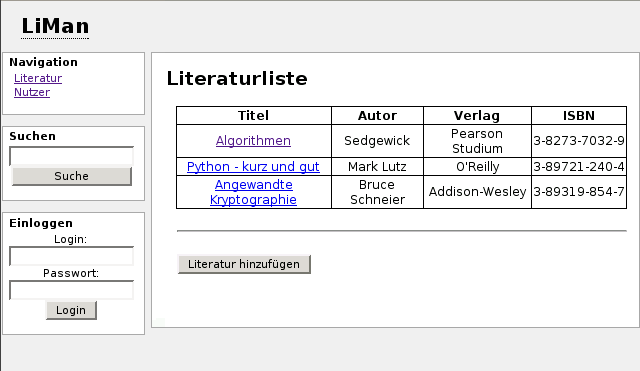
\includegraphics[scale=0.6]{index.png}

Hier ist die verf"ugbare Literatur aufgelistet. Durch Klicken der Titel gelangt man zur Detailansicht f"ur 
das jeweilige Buch. Mit dem Knopf am Ende der Liste (und entsprechenden Rechten) kann man Literatur hinzuf"ugen.

\subsubsection{Literaturdetails}
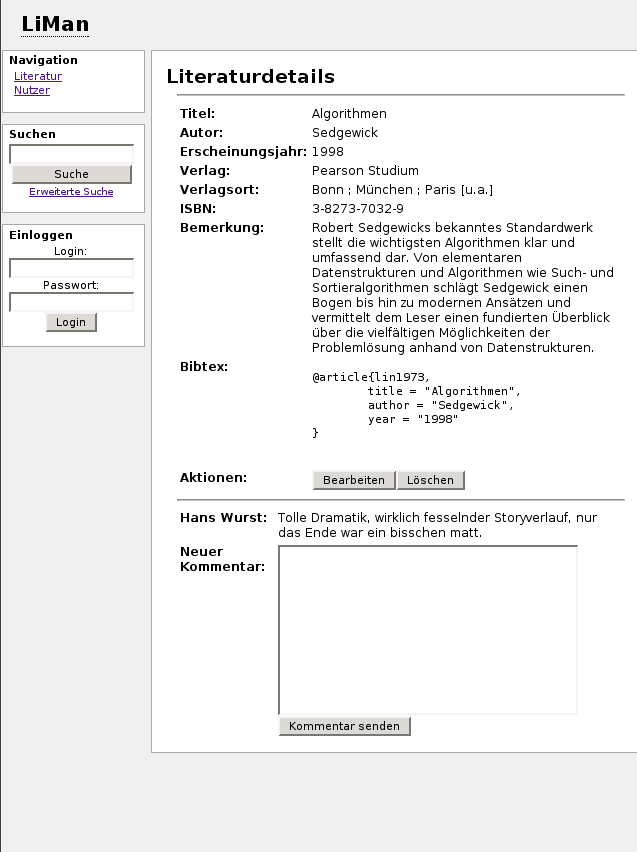
\includegraphics[scale=0.6]{lit.png}

Alle verf"ugbaren Information zum Buch werden hier aufgelistet. Hat man entsprechende Privilegien kann man auch
Bearbeiten/l"oschen oder Kommentare hinzuf"ugen/l"oschen.

\subsubsection{Literatur bearbeiten/hinzuf"ugen}
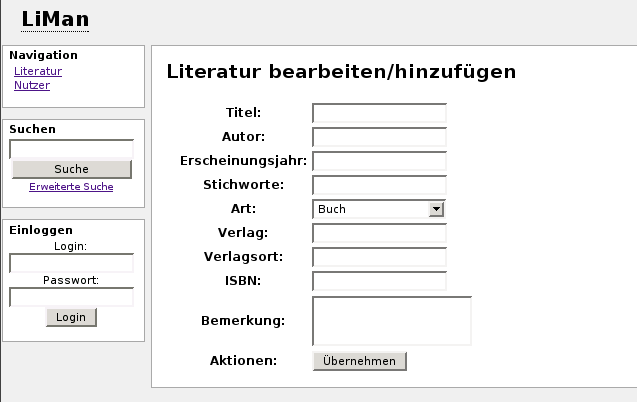
\includegraphics[scale=0.6]{litmod.png}

Hier kann Literatur bearbeitet oder hinzugef"ugt werden. Die Art der Literatur ist "uber eine Selectbox ausw"ahlbar.
Mehrere Autoren werden durch Kommata getrennt.
\newpage
\subsubsection{Erweiterte Suche}
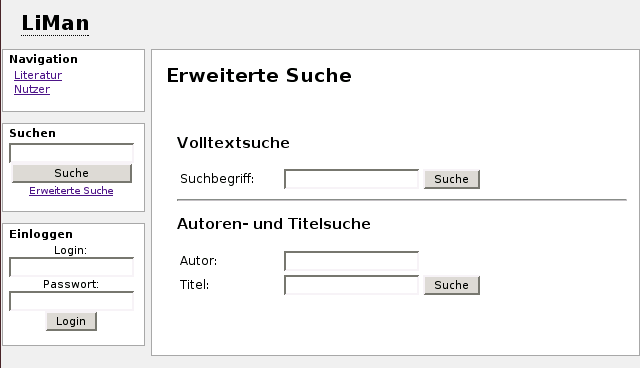
\includegraphics[scale=0.6]{searchmore.png}

Der Benutzer kann wahlweise "uber das Formular ``Volltextsuche'' analog zu der Suche in der Navigation suchen, oder die Suche
in dem Formluar ``Autoren- und Titelsuche'' auf Titel und/oder Autor beschr"anken.
\subsubsection{Suchergebnisse}
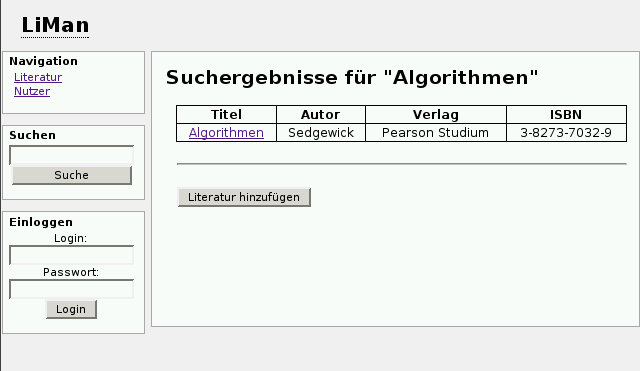
\includegraphics[scale=0.6]{search.png}

Das Ergebnis der Suche ist eine Literaturliste und wird entsprechend genauso bedient.

\subsubsection{Nutzerliste}
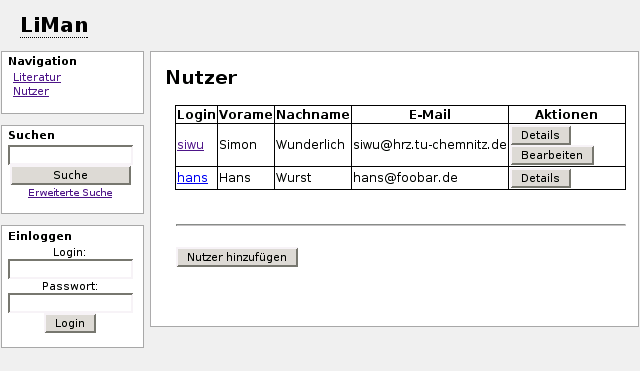
\includegraphics[scale=0.6]{user.png}

Hier werden alle Nutzer des Systems angezeigt, je nach Privilegien k"onnen auch die eigenen Daten oder andere
Daten modifiziert oder hinzugef"ugt werden.

\subsubsection{Nutzer bearbeiten/hinzuf"ugen}
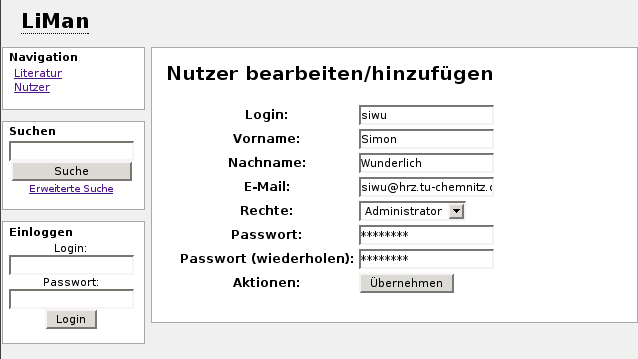
\includegraphics[scale=0.6]{usermod.png}

Hier werden nutzerspezifische Daten und das Passwort ge"andert. Die Rechtevergabe steht nur zur Auswahl wenn
der angemeldete Nutzer selbst Administrator ist.

\chapter{Spezifikation der operationellen Anforderungen}
\section{Operationelle Anforderungen an die Daten und Datenbasen}
Für die Abschätzung des Speicherplatzbedarfes für Daten und Speicher wird von den Annahmen ausgegangen,
dass für die Speicherung von in der Regel (bis auf wenige Ausnahmen, für die das gesondert vermerkt ist)\\
         gZahl - 2Byte, rZahl - 4 Byte\\
         Zeichenkette - 1Byte pro Zeichen (der maximalen Länge) erforderlich sind.

\begin{longtable}{|l|p{6.0cm}|p{2cm}|}
\hline
Element & Struktur & Bytes\\
\hline\hline
\endhead

Literatur & @Literatur\_Nr + Art + Titel + (Jahr) + (Verlag) + (ISBN) + (Beschreibung) + (Ort) + (Stichworte) & $24 + 20 + 40 + 2 + 40 + 20 + 250 + 40 + 100 = 546$ \\
\hline
Literatur\_Nr & gZahl *6stellig, 000001 $\leq$ Literatur\_Nr $\leq$ 999999*  & $4$\\
\hline
Art & ['' Sachbuch'' | '' Zeitschrift '' | '' wissenschaftliche Arbeit '' | ''Lehrbuch ''] & $24$\\
\hline
Titel & Zeichenkette40 & $40$ \\
\hline
Jahr & gZahl *4stellig* & $2$\\
\hline
Verlag & Zeichenkette40 & $40$ \\
\hline
ISBN & Zeichenkette20 & $20$  \\
\hline
Beschreibung & Zeichenkette250 & $250$ \\
\hline
Ort & Zeichenkette40 & $40$ \\
\hline
Stichworte & Zeichenkette100 & $100$\\
\hline\hline

Autor & @Autor\_Nr + Autorname & $4 + 40 = 44  $\\
\hline
Autor\_Nr & gZahl *6stellig, 000001 $\leq$ Autor\_Nr $\leq$ 999999* & $4$ \\
\hline
Autorname & Zeichenkette40 & $40$\\
\hline\hline

Kommentar & @Kommentar\_Nr + Kommentartext + Literatur\_Nr + Mitglieds\_Nr & $4 + 400 + 4 + 4 = 412 $\\
\hline
Kommentar\_Nr & gZahl *6stellig, 000001 $\leq$ Kommentar\_Nr $\leq$ 999999* & $4$ \\
\hline
Kommentartext & Zeichenkette400 & $400$\\
\hline

Mitglied  & @Mitglieds\_Nr  + Name + Vorname + Login + Passwort + Rechte + E-Mail & $4 + 20 + 20  + 12 + 12 + 13 + 350 = 431 $\\
\hline
Mitglieds\_Nr & gZahl *6stellig, 000001 $\leq$ Benutzer\_Nr $\leq$ 999999* & $4$ \\ 
\hline
Name & Zeichenkette20 & $20$\\
\hline
Vorname & Zeichenkette20 & $20$ \\
\hline
E-Mail & Zeichenkette350 & $350$ \\
\hline
Login & Zeichenkette12 & $12$\\
\hline
Passwort & Zeichenkette12 & $12$\\
\hline
Rechte & [``Benutzer'' $\mid $``Administrator``] & $13$ \\
\hline\hline

Mitgliedsdaten & Name + Vorname + Login + Passwort + Rechte + E-Mail& $20 + 20 + 12 + 12 + 13 + 350 = 427 $\\
\hline
Literaturdaten & Art + Titel + Autorname + (Jahr) + (Verlag) + (ISBN) + (Beschreibung) + (Ort) + (Stichworte) & $24 + 40 + 40 + 2 + 40 + 20 + 250 + 40 + 100 = 556 $ \\
\hline
Kommentardaten & Literatur\_Nr + Mitglieds\_Nr + Kommentartext & $4 + 4 + 4 = 12 $ \\
\hline
BibTeX-Datei & *Datei im Bibtexformat* & $1024$\\
\hline
Suchbegriff & Zeichenkette100 & $100 $ \\
\hline
Exportanfrage & Literatur\_Nr & $4 $ \\
\hline\hline

Bestätigung\_BibTeXImport & Literatur\_Nr + Zeichenkette ''Importieren vorgenommen`` & $4 + 23 = 27 $\\
\hline
Bestätigung\_Literaturanlegen & Literatur\_Nr + Zeichenkette ''Anlegen vorgenommen`` & $4 + 19 = 23 $\\
\hline
Bestätigung\_Literaturändern & Literatur\_Nr + Zeichenkette ''Änderung vorgenommen`` & $4 + 20 = 24$ \\
\hline
Bestätigung\_Literaturlöschen & Literatur\_Nr + Zeichenkette ''Löschen vorgenommen`` & $4 + 19 = 23 $\\
\hline
Bestätigung\_Kommentaranlegen & Kommentar\_Nr + Zeichenkette ''Anlegen vorgenommen`` & $4 + 19 = 23 $\\
\hline
Bestätigung\_Kommentarändern & Kommentar\_Nr + Zeichenkette ''Änderung vorgenommen`` & $4 + 20 = 23$\\
\hline
Bestätigung\_Kommentarlöschen & Kommentar\_Nr + Zeichenkette ''Löschen vorgenommen`` & $4 + 19 = 23$ \\
\hline
Bestätigung\_Mitgliedanlegen & Mitglieds\_Nr + Zeichenkette ''Anlegen vorgenommen`` & $4 + 19 = 23 $ \\
\hline
Bestätigung\_Mitgliedändern & Mitglieds\_Nr + Zeichenkette ''Änderung vorgenommen`` & $4 + 20 = 24$\\
\hline
Bestätigung\_Mitgliedlöschen & Mitglieds\_Nr + Zeichenkette ''Löschen vorgenommen`` & $4 + 19 = 23$\\
%\hline
%Literatur\_Info & Literatur + Kommentare & $ 549 + 412 = 961 $ \textbf{KOMMENTARE = VIELE KOMMENTARE UND NICHT NUR EINER}\\
\hline
Suchtreffer & \{Literatur\_Nr + Titel + Verlag + ISBN\} & $4 + 40 + 40 + 20 = 104$\\
\hline
Letzte\_Literatur & \{Literatur\_Nr + Titel + Autorname + Verlag + ISBN\} & $4 + 40 + 40 + 40 + 20 = 144$\\
\hline
Mitgliederliste & \{Mitglieds\_Nr + Name + Vorname\} & $4 + 20 + 20 = 44 $\\
\hline
\end{longtable}


\subsection{Speicher (Angaben zum Speicherbedarf in Byte)}
\begin{tabular}[ht]{|l|l|l|l|l|}
\hline
Speicher & Struktur & Minimum & Mittel & Maximum \\
\hline\hline
Literatur & {Literatur} & $0*556$ & $50*556=27800$ & $100*556=55600$ \\
Kommentare & {Kommentar} & $0*412$ & $50*412=20600$ & $100*412=41200$ \\
Mitglieder & {Mitglied}  & $0*431$ & $50*431=21550$ & $100*431=43100$ \\
Autoren & {Autor} & $1*44$ & $2*44=88$ & $5*44=220$ \\ 
\hline
\end{tabular}

\subsection{Weitere Datenflüsse}
\begin{tabular}[ht]{|l|p{4cm}|p{2cm}|p{2cm}|p{2cm}|}
\hline
Datenfluss & Struktur & Minimum & Mittel & Maximum \\
\hline\hline

Suchtreffer & \{Literatur\_Nr + Titel + Verlag + ISBN\}  & $0*104$ & $50*104=5200$ & $100*104=10400$ \\
Letzte\_Literatur & \{Literatur\_Nr + Titel + Autor + Verlag + ISBN\}  & $0*144$ & $50*144=7200$ & $100*144=14400$ \\
BibTeX-Datei & \{Datei im Bibtexformat\} & $0*1024$ & $50*1024=51200$ & $100*1024=102400$ \\
Literatur\_Info & \{Literatur + Kommentare\} & $546 + 0*412=546$ & $546 + 100*412=41746$ & $546 + 200*412=82946$ \\
\hline
\end{tabular}

\subsection{Abschätzungen}
\begin{itemize}
 \item \textbf{Gesamtsystem}: Als Nutzungszeit wird von 5 Jahren ausgegangen, wobei die maximale Nutzungszeit, 
die an das System gestellt wird, 10 Jahre betr\"agt.
 \item \textbf{Mitglieder}: Es wird erwartet, dass nicht mehr als 500 Mitglieder den Dienst in Anspruch nehmen werden. Im Durchschnitt wird
 die Mitgliederzahl etwa 200 betragen.
\item \textbf{Leistungen}: Bei einem Stundenaufkommen zwischen 20 und 30 Stunden pro Jahr, kann davon ausgegangen werden, dass jedes 
Mitglied in etwa 53 Suchanfragen, 10 Literatureinstellung und 20 Kommentaren abgibt. Die Informationen bleiben erhalten, solange der Dienst existiert.  
\item \textbf{Exportieren}: In einem Jahr werden ca. 100 bis 150 Exportanfragen pro Mitglied erwartet.
\end{itemize}

\subsection{Genauigkeit}
Es werden nur Ganzzahlen im ganzen System verarbeitet. Es werden hierbei keine problematische Rechnungen vorgenommen.

\section{Operationelle Anforderungen an die Datenströme}
Umfangreiche Datenstr\"ome k\"onnen im System nur auftreten, wenn Suchanfragen gestellt, Letzte Literatur aufgerufen oder eine BibTex-Datei abgefragt wird. 
Diese Datenstr\"ome bewegen sich im Bereich von maximal 1 Megabyte und im Durchschnitt 30 Kilobyte, sodass es selten
zu gr\"o\"seren Datenstr\"omen kommt.


\section{Operationelle Anforderungen an die Prozesse}
Es wird von Antwortzeiten bis zu 2 Sekunden gerechnet. Da die meisten Prozesse auf dem Server verarbeitet werden und der Client diese nur Darstellen muss, 
kann von 2 Sekunden ausgegangen werden. 

\chapter{Spezifikation wichtiger Qualitätsanforderungen}
\section{Benutzerbarkeit}
TODO siehe Beispielbeleg S. 24

\section{Zuverlässigkeit}
TODO siehe Beispielbeleg S. 24

\section{Integrität}
TODO siehe Beispielbeleg S. 24

\section{Flexibilität}
TODO siehe Beispielbeleg S. 24

\section{Portabilität}
TODO siehe Beispielbeleg S. 24
\chapter{Basismaschine und Entwicklungsumgebung}
\section{Basismaschine}
\subsection{Hardwarekonfiguration}
F"ur {\bf Webserver} wird folgende Ausstattung ben"otigt:
\begin{itemize}
 \item Server (Monitor)
 \item Breitband-Netzwerk (z.B. SDSL, Ethernet)
 \item 5 MB Festplattenspeicher
\end{itemize}
Als notwendige Minimalausstattung des für den {\bf Nutzer-PC} wird vorgeschlagen:
\begin{itemize}
 \item Basis-PC (Tastatur, Maus, 15" Farbmonitor)
 \item Netzwerk (z.B. Modem, Ethernet)
\end{itemize}
Da die Nutzung des Systems komplett Serverseitig funktioniert wird auf dem Nutzer-PC kein Festplattenspeicher verbraucht, da die
Bedienung komplett "uber den Webbrowser erfolgt. Eine schnelle CPU und eine breitbandige Netzwerkverbindung
kann den Arbeitskomfort zus"atzlich verbessern.


\subsection{Betriebssystem}
Webserver:
\begin{itemize}
\item Unix oder Unix-kompatibel
\end{itemize}
Nutzer-PC:
\begin{itemize}
\item Windows ab Windows 95
\item Linux oder Unix-kompatibel
\item MacOS
\item PalmOS
\end{itemize}

\subsection{Sonstige Basissoftware}
Webserver:
\begin{itemize}
\item MySQL 5.0
\item Apache 2.0
\item PHP 5.1
\end{itemize}
Nutzer-PC:
\begin{itemize}
\item Webbrowser, z.B. Firefox, Konqueror, Opera, Internet Explorer
\end{itemize}


\section{Entwicklungsumgebung}
Es wird ein normaler Texteditor verwendet (z.b. vim, emacs).

\chapter{Planung}
\section{Gantt-Diagramm}
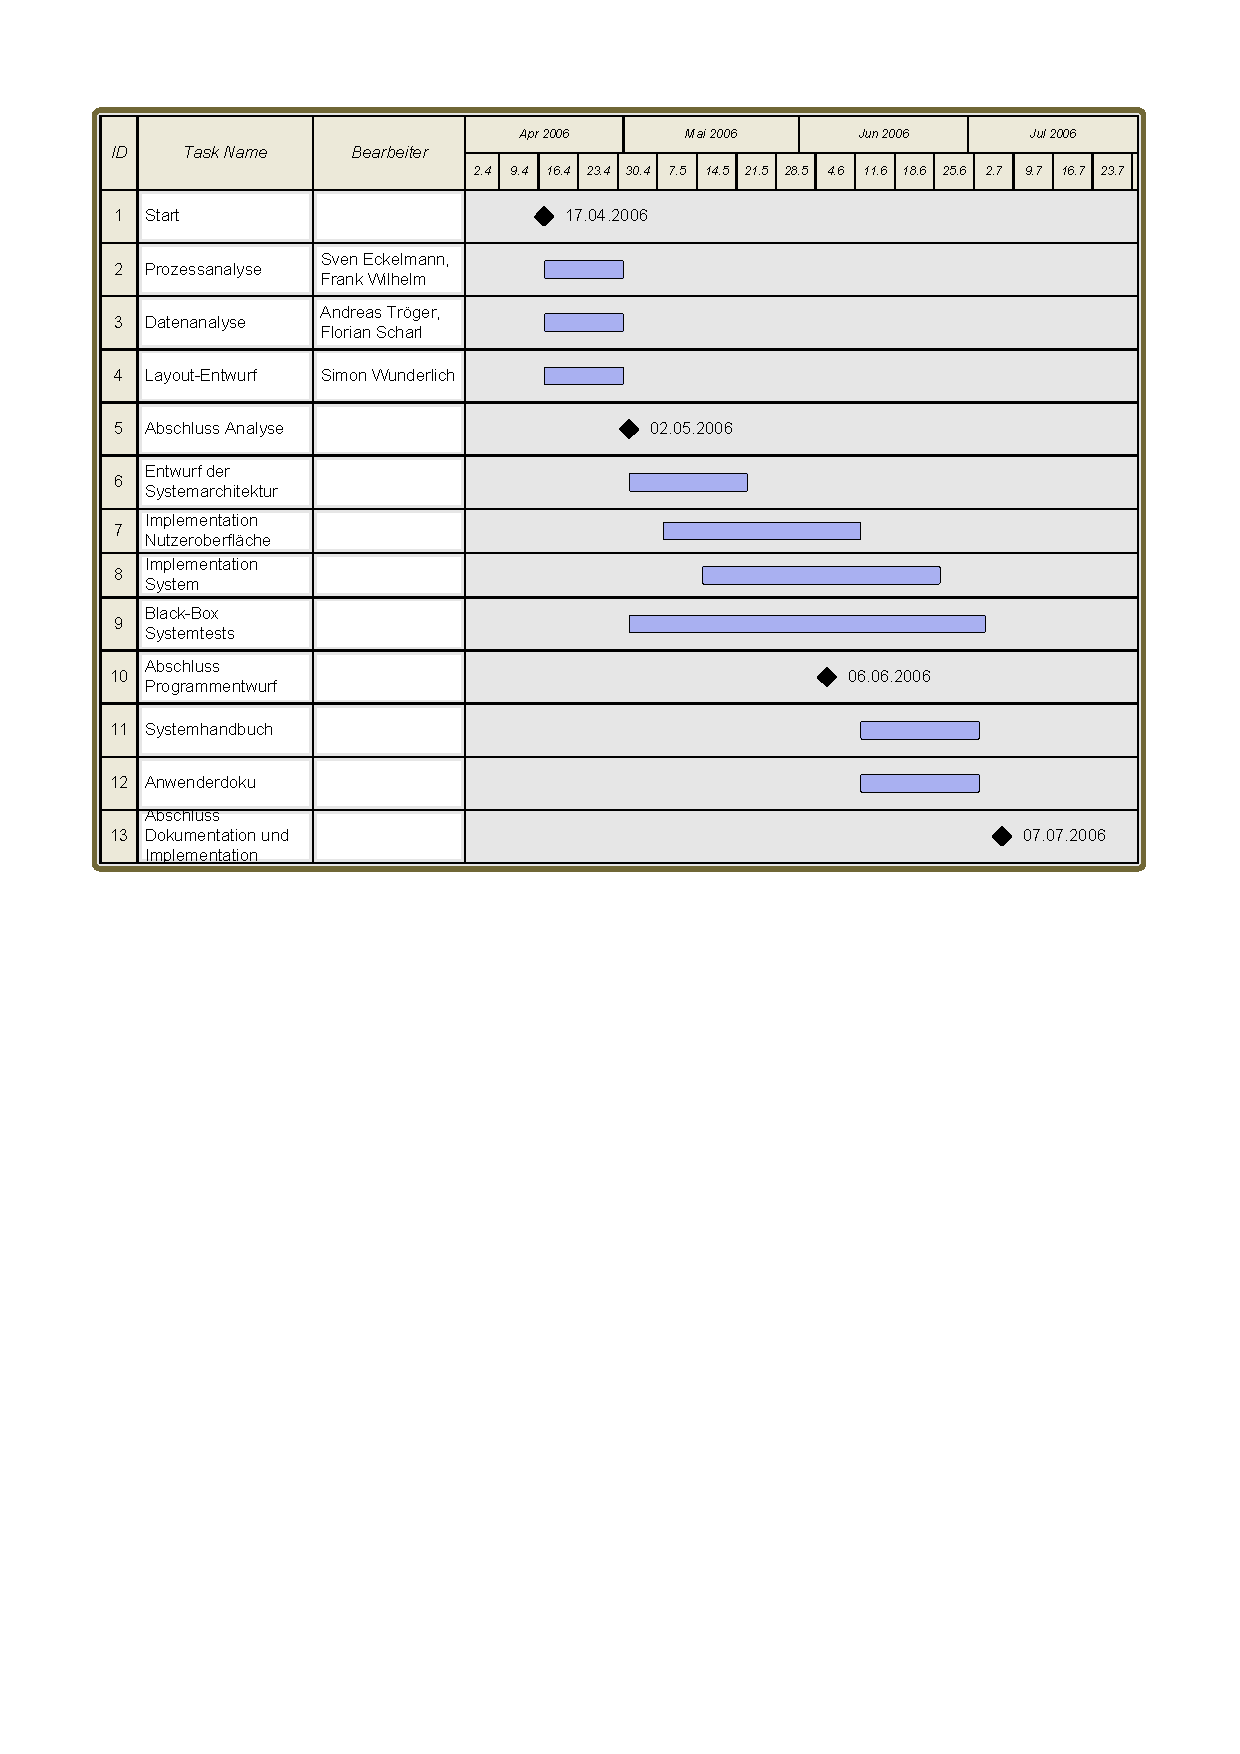
\includegraphics[scale = 0.93, bb = 1.5cm 14.8cm 19.4cm 28cm]{ganttchart}

\end{document}
